\clearpage
\section{Quantum Noise}

\subsection*{Introduction}\label{sec:intro}


This document describes an emission and detection system which is used to simulate the effects of quantum noise.
\\
\\
This system is based in the transmission of coherent states as the support for information. The following section introduces some aspects about coherent states, with special focus on quantum noise.\\
\\
A coherent state is a sobreposition of photon number states ($\ket{n}$), which is generated by a single-mode laser.
\footnote{Loudon, p.190}
A coeherent state with expected value $\alpha$ is discribed by the following state:
$$
\ket{\alpha} = e^{-\frac{|\alpha|^2}{2}} \sum_{n=0}^\infty \frac{\alpha^n}{\sqrt{n!}} \ket{n}
$$
in which $\ket{\alpha}$ is a photon number state.
\footnote{Loudon, p.184}
A Fock state represents a state with $n$ excitations?, that in the current case corresponds to photons. We also have creation ($\hat{a}^\dagger$) and anihiliaton ($\hat{a}$) operators which add and remove one photon from the Fock states:????$$
\hat{a} \ket{n} = \sqrt{n} \ket{n-1} \qquad \qquad \hat{a}^\dagger \ket{n} = \sqrt{n+1} \ket{n+1}
$$
The coherent state is an eigenstate of the annihilation operator, $\hat{a}\ket{\alpha} = \alpha \ket{\alpha}$.\\
We can define two new operators,  $X$ and $Y$, that are quadrature operators
\footnote{Loudon, p.138, (4.3.36)}
defined as: (TALVEZ FALAR UM POUCO SOBRE O EFEITO DISTO NAS MEDICOEES REAIS)
$$
\hat{X} = \frac{1}{2} \left( \hat{a}^\dagger + \hat{a} \right) \qquad \qquad
\hat{Y} = \frac{i}{2} \left( \hat{a}^\dagger - \hat{a} \right)
$$
\\
The expected value of these two operators, using a coherent state $\ket{\alpha}$ are:
$$
\braket{\hat{X}} = \textrm{Re}(\alpha) \qquad \qquad
\braket{\hat{Y}} = \textrm{Im}(\alpha)
$$
We see then that these operator give us the real and imaginary part of $\alpha$.\\
Now, we can obtain the uncertainty of these operators, using:
$$
\textrm{Var}(\hat{X}) = \braket{\hat{X}^2} - \braket{\hat{X}}^2
$$
(VALERA A PENA GENERALIZAR A QUADRATURA?)\\
For each of these quadrature operators the variance will be:
$$
\textrm{Var}(\hat{X}) = \textrm{Var}(\hat{Y}) = \frac{1}{4}
$$
This result show us that the variance of measuring in any quadrature is the same and independent of the value of $\alpha$.\\
\\
The manifestation of this noise is made in the act of measurement (CONFIRMAR).\\
(REVER A QUESTAO DA DETECCAO COM PHOTODIODES)\\
\\
Besides this limitation, we also have shot noise introduced by the photodiodes????
%
%
%
%
%This document describes an emission and detection system that uses coherent states as it's means?? of transmission???.\\
%The transmitted information consists in a binary sequence which is ??translated?? in a sequence of coherent states. In this simulation, the used constellation is formed by the states $\{ \ket{\alpha}, \ket{i\alpha}, \ket{ - \alpha}, \ket{ - i \alpha} \}$, in which $\alpha$ is defined as $\braket{n} = |\alpha|^2$ ($\braket{n}$ is the expected number of photons in a state). (METER MELHOR) \\
%\\
%One of the main effects studied in this system is quantum noise, which is an intrinsic effect?? to coherent states(VER MARK FOX). In principle???? (VER REFERENCIAS) the variance of a coherent state is given by $\Delta X_1 \Delta X_2 = \frac{1}{4}$.\\
%\\
%But, given that we combine two photocurrents to obtain an output current, then the total noise will have a combined value of SOMETHING??? Procurar referencias.\\
%\\
%Therefore, assuming Gaussian?? (WHY GAUSSIAN?) shot noise, for each quadrature we want $\textrm{Var}(X_i) = \frac{1}{4}$ ?????\\
%(TENHO DE PROCURAR REFERENCIAS)
%\\
%\\
%In this simulation, we introduce quantum noise in the photodiodes.
%We know that a coherent state has an expected number of photons distributed by a Poisson distribution, which has an average number equal to it's variance. Therefore, when the photodiode detects the power of signal, which is proportional to the number of photons, then it's variance must also be proportional to the number of photons.\\
%\\
%In fact the last step in detecting the resulting signal introduces an difference between currents, but that only will increase the variance. Assuming the independence between detections, and it's intrinsic noise (PROCURAR MELHOR PALEIO), then:
%$$
%\textrm{Var}(I_{out}) = \textrm{Var}(I_1) + \textrm{Var}(I_2)
%$$
%Therefore, the best result we can achieve will be $\textrm{Var}(X) = \frac{1}{4}$ ???? (PROCURAR PALEIO SOBRE ISTO)\\
\\
\\
\subsection*{Functional Description}

The simulation setup is described by diagram in figure \ref{fig:setup}. We start by generating a state from one of the four available ones.???? Then, the signal is received in a Hybrid Detector??? where the signal is compared with a local oscillator giving four different signals in it's output. Two of those signals are detected by a photodiode which output will be the difference of the two photocurrents. The other two signals will be also be detected by another photodiode, which will obtain the other quadrature of the signal.????? (TEM QUE FICAR MELHOR EXPLICADO).



\begin{table}[H]
\centering
\begin{tabular}{c|c}
System Blocks          & netxpto Blocks       \\ \hline
- & MQAM \\
- & LocalOscillator \\
- & Hybrid?? \\
- & Photodiode??\\
- & Sampler ??\\
\end{tabular}
\end{table}


\begin{figure}[h]
\centering
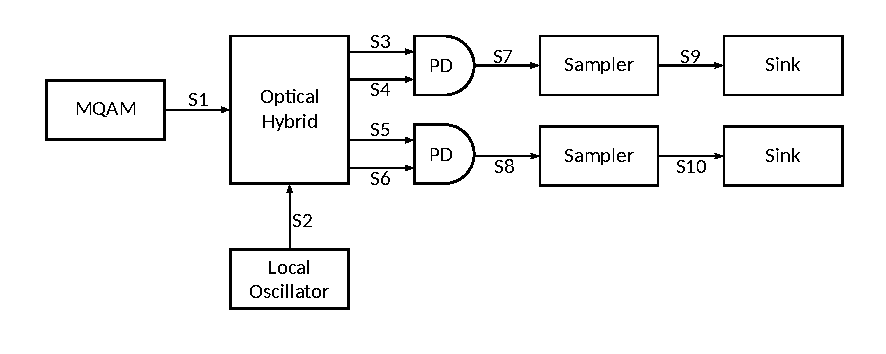
\includegraphics[width=\linewidth]{./sdf/quantum_noise/figures/scheme1.pdf}
\caption{Overview of the optical system being simulated.}
\label{fig:setup}
\end{figure}


\subsection*{Required files}\label{Required files}

Header Files
\begin{table}[H]
\centering
\begin{tabulary}{1.0\textwidth}{|L|L|}
\hline
\textbf{File}           & \textbf{Description}                           \\
\hline
netxpto.h               & Generic purpose simulator definitions.         \\
\hline
m\_qam\_transmitter.h   & ---\\
\hline
local\_oscillator.h     & Generates continuous coherent signal.            \\
\hline
optical\_hybrid.h       & ---\\
\hline
photodiode.h            & ---\\
\hline
sampler.h               & ---\\
\hline
sink.h                  & Closes any unused signals.                       \\
\hline
\end{tabulary}
\end{table}
%
%
Source Files
\begin{table}[H]
\centering
\begin{tabulary}{1.0\textwidth}{|L|L|}
\hline
\textbf{File}                   & \textbf{Description}\\
\hline
netxpto.cpp                     & Generic purpose simulator definitions.\\
\hline
m\_qam\_transmitter.cpp         & ---\\
\hline
local\_oscillator.cpp           & Generates continuous coherent signal.\\
\hline
optical\_hybrid.cpp             & ---\\
\hline
photodiode.cpp                  & ---\\
\hline
sampler.cpp                     & ---\\
\hline
sink.cpp                        & Closes any unused signals.\\
\hline
\end{tabulary}
\end{table}


\subsection*{System Input Parameters}

This system takes into account the following input parameters:
\begin{table}[H]
\centering
\begin{tabulary}{1.0\textwidth}{|C|L|}
\hline
\textbf{System Parameters} & \textbf{Description}\\
\hline
numberOfBitsGenerated   & Gives the number of bits to be simulated\\
\hline
bitPeriod               & Sets the time between adjacent bits\\
\hline
wavelength              & Sets the wavelength of the local oscillator in the MQAM????\\
\hline
samplesPerSymbol        & Establishes the number of samples each bit in the string is given\\
\hline
localOscillatorPower1   & Sets the optical power, in units of W, of the local oscillator inside the MQAM\\
\hline
localOscillatorPower2   & Sets the optical power, in units of W, of the local oscillator used for Bob's measurements\\
\hline
localOscillatorPhase    & Sets the initial phase of the local oscillator used in the detection\\
\hline
transferMatrix          & Sets the transfer matrix of the beam splitter used in the homodyne detector\\
\hline
responsivity            & Sets the responsivity of the photodiodes used in the homodyne detectors\\
\hline
bufferLength            & Sets the length of the buffer used in the signals\\
\hline
iqAmplitudeValues       & Sets the amplitude of the states used in the MQAM????\\
\hline
shotNoise               & Chooses if quantum shot noise is used in the simulation\\
\hline
samplesToSkip			& Sets the number of samples to skip when writing out some of the signal files.\\
\hline
\end{tabulary}
\end{table}		

\subsection*{Inputs}

This system takes no inputs.

\pagebreak
\subsection*{Outputs}

The system outputs the following objects:
\begin{itemize}
\item Signals:
\begin{itemize}
\item Binary Sequence used in the MQAM; (S$_{0}$)
\item Local Oscillator used in the MQAM; (S$_{1}$)
\item Local Oscillator used in the detection; (S$_{2}$)
\item Optical Hybrid Outputs; (S$_{3}$, S$_{4}$, S$_{5}$, S$_{6}$)
\item In phase Photodiode output; (S$_{7}$)
\item Quadrature Photodiode output; (S$_{8}$)
\item In phase Sampler output; (S$_{9}$)
\item Quadrature Sampler output; (S$_{10}$)
\end{itemize}
\end{itemize}	

\subsection*{Simulation Results}\label{subsec:SHresults}

The objective of this simulation was to get the (quantum noise???) associated to the detection of coherent states.\\
\\
\begin{figure}[h]
\centering
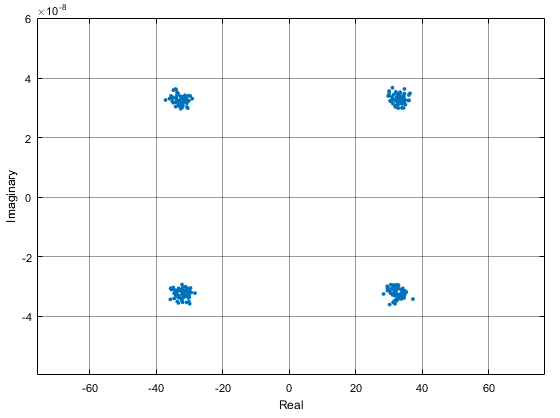
\includegraphics[width=10cm]{./sdf/quantum_noise/figures/constelation1.png}
\caption{Simulation of a constelation of 4 states (n = 100)}
\label{fig:constelation}
\end{figure}
\\
We expect that the variance is invariant with the number of photons sent from Alice. The plot in \ref{fig:variance} show that the simulation also shows this invariance with the number of photons.\\
\begin{figure}[H]
\centering
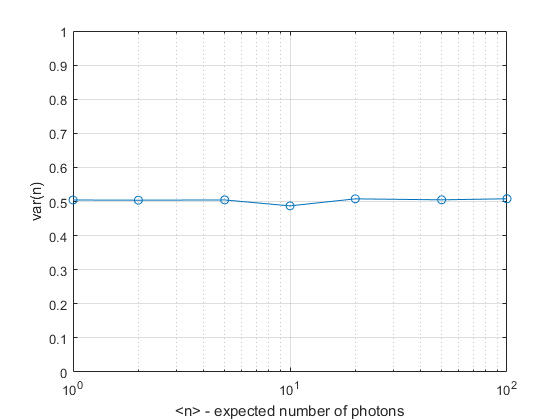
\includegraphics[width=10cm]{./sdf/quantum_noise/figures/variance_n.png}
\caption{Simulation of the variance of $n$.}
\label{fig:variance}
\end{figure}
We can conclude that the expected variance will give us $\textrm{Var(X)} = \frac{1}{2}$.\\
The results obtained in our simulations are in accordance with the theoretical prevision???


%\subsection*{Block Description}
%
%\subsubsection*{MQAM mapper???}
%\subfile{../../lib/tex/m_qam_mapper_v2}
%
%\subsection{Local Oscillator}
%\subfile{../../lib/tex/localoscillator}
%1
%\subsection{Optical Hybrid}
%MISSING FILE FOR OPTICAL HYBRID\\
%%\subfile{../../lib/tex/beamsplitter}
%
%\subsection{Photodiode}
%\subfile{../../lib/tex/photodiode}
%
%\subsection{Sampler}
%\subfile{../../lib/tex/sampler}

\subsection*{Known Problems}
\begin{enumerate}
    \item ----
\end{enumerate}

